\section{Aplicativo Backup}

Para lidar com o caso de indisponibilidade do controlador local Morpheus, da rede local (roteador \emph{wireless}) ou da conexão com a Internet, foi desenvolvido um aplicativo de \textit{backup}. Esse aplicativo permite acesso direto ao módulo através do endereço local (supondo que o dispositivo celular esteja na mesma rede) ou por conexão direta com o ponto de acesso do módulo (disponível todo o tempo ou sempre que o módulo não consiga conexão com a Internet, a depender da preferência do usuário).

\subsection{Requisitos}

Destacam-se os requisitos mais críticos do aplicativo backup:

\begin{enumerate}
	\item Permitir acesso direto ao módulo em caso de indisponibilidade da rede Wi-Fi e Internet;
	\item Permitir a visualização de estado de sensores e a atuação em tempo próximo ao apresentado por botão físico;
	\item Acesso ao módulo por meio de endereço local no caso de haver rede local disponível, mas sem acesso à Internet;
	\item Possibilitar ao usuário configurar rede Wi-Fi, nome do módulo, cor do painel, offset de sensores, nome dos relés e regras de atuação (por radiofrequência, com senha ou não, por horário, por eventos dos sensores de presença e abertura, além do tempo em que deve ficar ligado no caso de configurações automáticas);
	\item Permitir configurar múltiplos códigos RF (radiofrequência) para sensor de abertura, atuação do relé 1 ou do relé 2;
	\item Permitir ao usuário configurar controle de acesso e senha para atuação de um relé em específico;
	\item Segregar permissões entre administrador e usuário --- usuários não podem executar configurações, somente visualizar estados e atuar em relés sem senha;
	\item Permitir visualização de vários módulos da residência;
	\item Ter interface de fácil navegação, intuitiva.
\end{enumerate}

\subsection{Tecnologias utilizadas}

Para o desenvolvimento do aplicativo backup, foram utilizados:

\begin{enumerate}
	\item Módulo como servidor, utilizando bibliotecas de comunicação próprias do ESP8266 no caso de comunicação direta com o módulo, e uso do módulo como cliente, usando a mesma biblioteca;
	\item Uso de \emph{ping} para verificação de conexões e execução de rotinas para a correta configuração de estado do ponto de acesso (ligado se não conectado à rede), rotinas de desconexão e reconexão;
	\item CSS para a implementação de interface amigável para o usuário, e segregação de configurações em níveis de navegação maiores para que configurações mais usadas sejam mais facilmente acessíveis a partir do menu principal do módulo;
	\item JavaScript para as rotinas de configuração e atualização do estado no menu principal;
	\item HTML5 para o desenvolvimento da maioria das páginas;
	\item EEPROM do módulo ESP8266, onde todas configurações de conexão, gerais e relés ficam armazenadas. Em caso de mudança desses parâmetros, ocorre sua persistência na EEPROM;
	\item Bibliotecas próprias para interface com sensores e outros periféricos (DHT e I2C, por exemplo), comunicação em geral, além do Wi-Fi e \emph{Access Point} (PubSub para comunicação por MQTT).
\end{enumerate}

\subsection{Navegação}

A partir da tela inicial, um cliente pode verificar todos os módulos presentes em sua casa, visualizar temperatura, umidade, luminosidade, sensores de presença ou abertura e apagar ou acender luzes (para atuadores protegidos com senha, o usuário deve acessar a página do respectivo módulo), numa interface configurável (o usuário pode configurar quais parâmetros observar nesse menu principal). A tela da Figura \ref{fig:telasPrincipaisBackup} é própria para celulares, enquanto a tela da Figura \ref{fig:plantaBackup}, com posicionamento configurável e que simula a planta de uma casa (em um cenário real, poderia ser a própria planta da casa do usuário) é própria para desktops.

\begin{figure}[H]
	\centering
	\caption{Telas principais do Aplicativo Backup}
  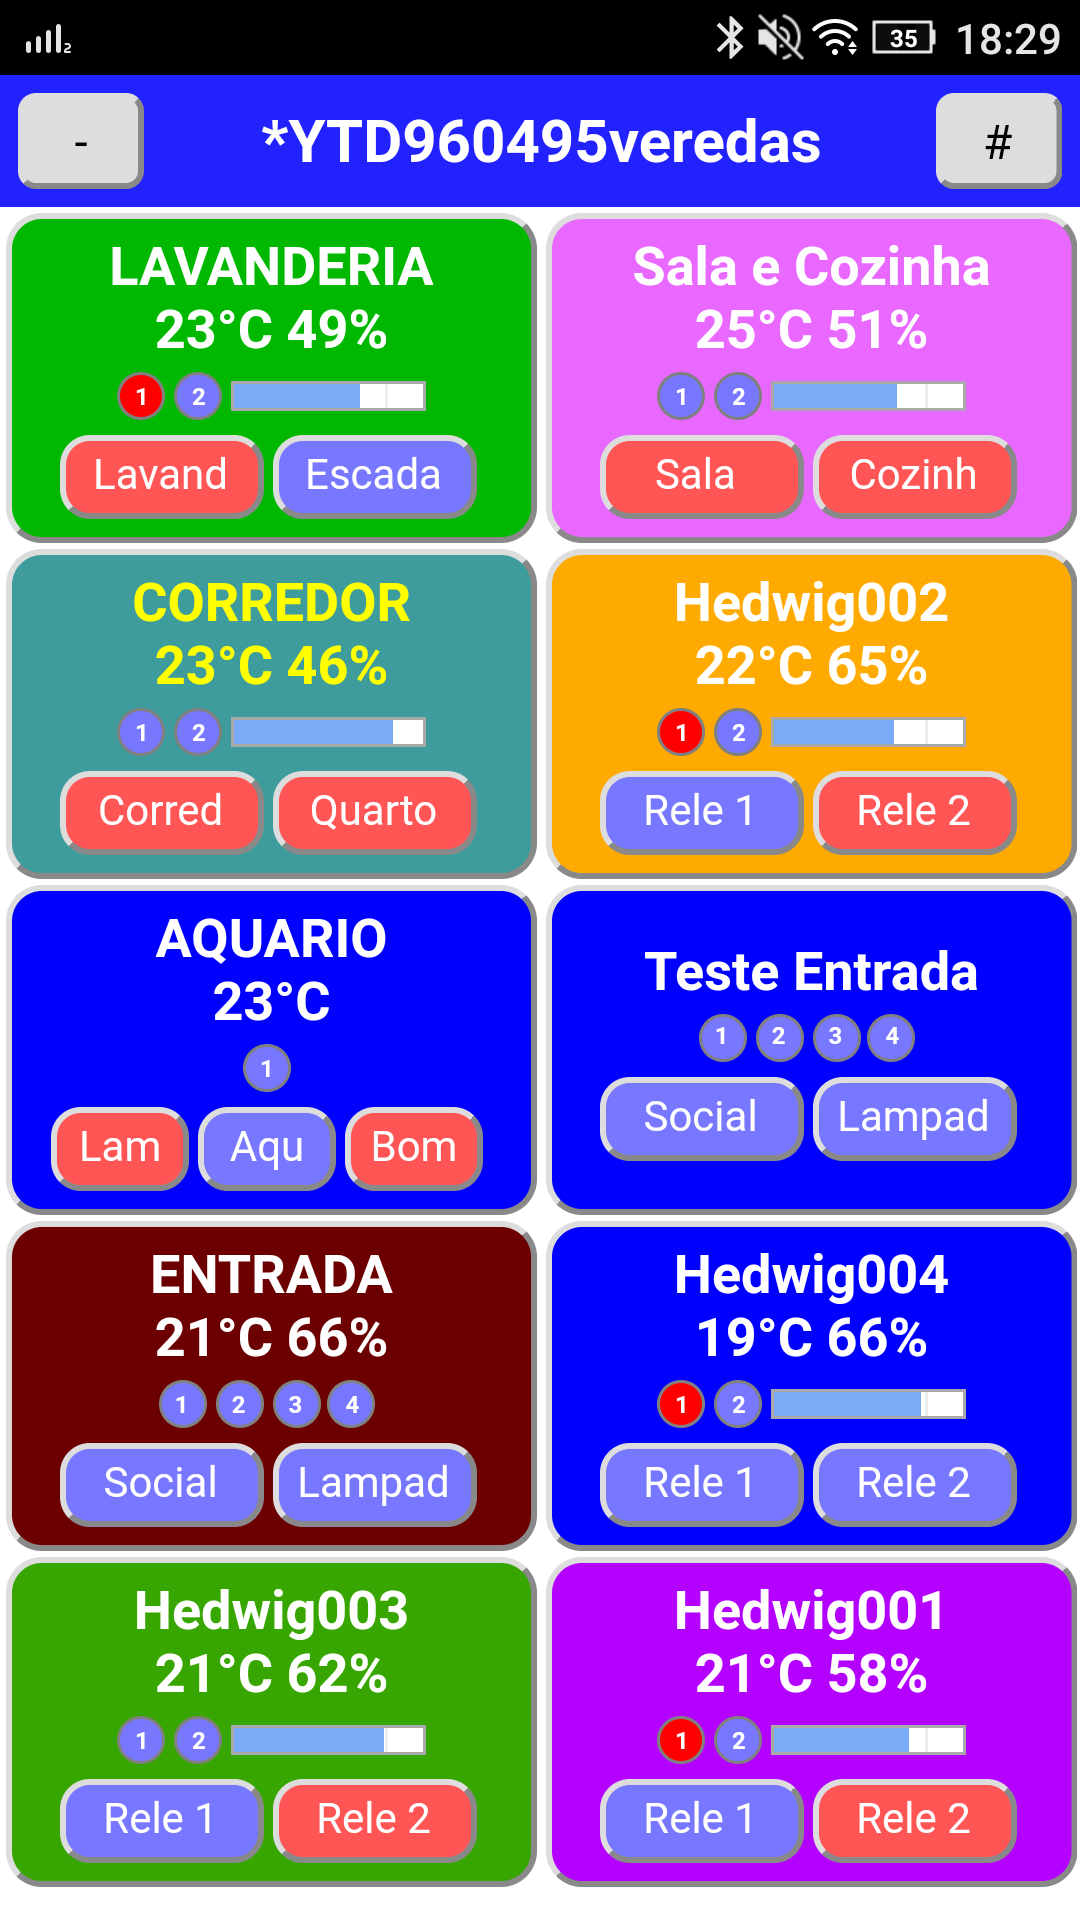
\includegraphics[width=0.5\textwidth]{telasPrincipaisBackup}
\label{fig:telasPrincipaisBackup}
\end{figure}

\begin{figure}[H]
  \centering
  \caption{Visão geral da planta de uma casa com o Aplicativo Backup}
  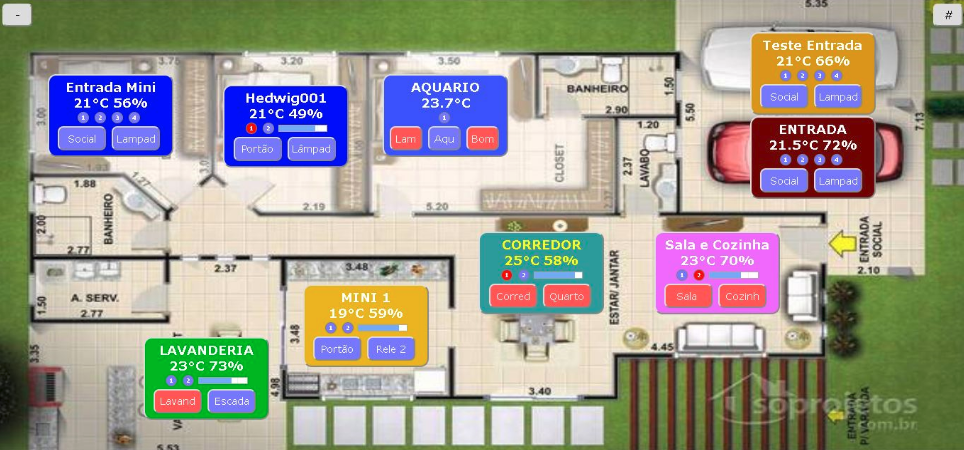
\includegraphics[width=0.8\textwidth]{plantaBackup}
  \label{fig:plantaBackup}
\end{figure}

A partir do menu principal, pode-se acessar o menu do módulo desejado (vide Figura \ref{fig:menuPrincipalBackup}). Nele, encontram-se informações de luminosidade, horário, data, temperatura, umidade, sensor de presença (sensor 1) e sensor de abertura (sensor 2), além de controle de portão, lâmpada ou eletrodoméstico. Também exibe o nível de recepção de Wi-Fi do módulo e a versão do \emph{firmware}.

\begin{figure}[hbp]
    \centering
    \begin{minipage}{.4\linewidth}
        \centering
        \captionof{figure}{Menu principal do Aplicativo Backup}
        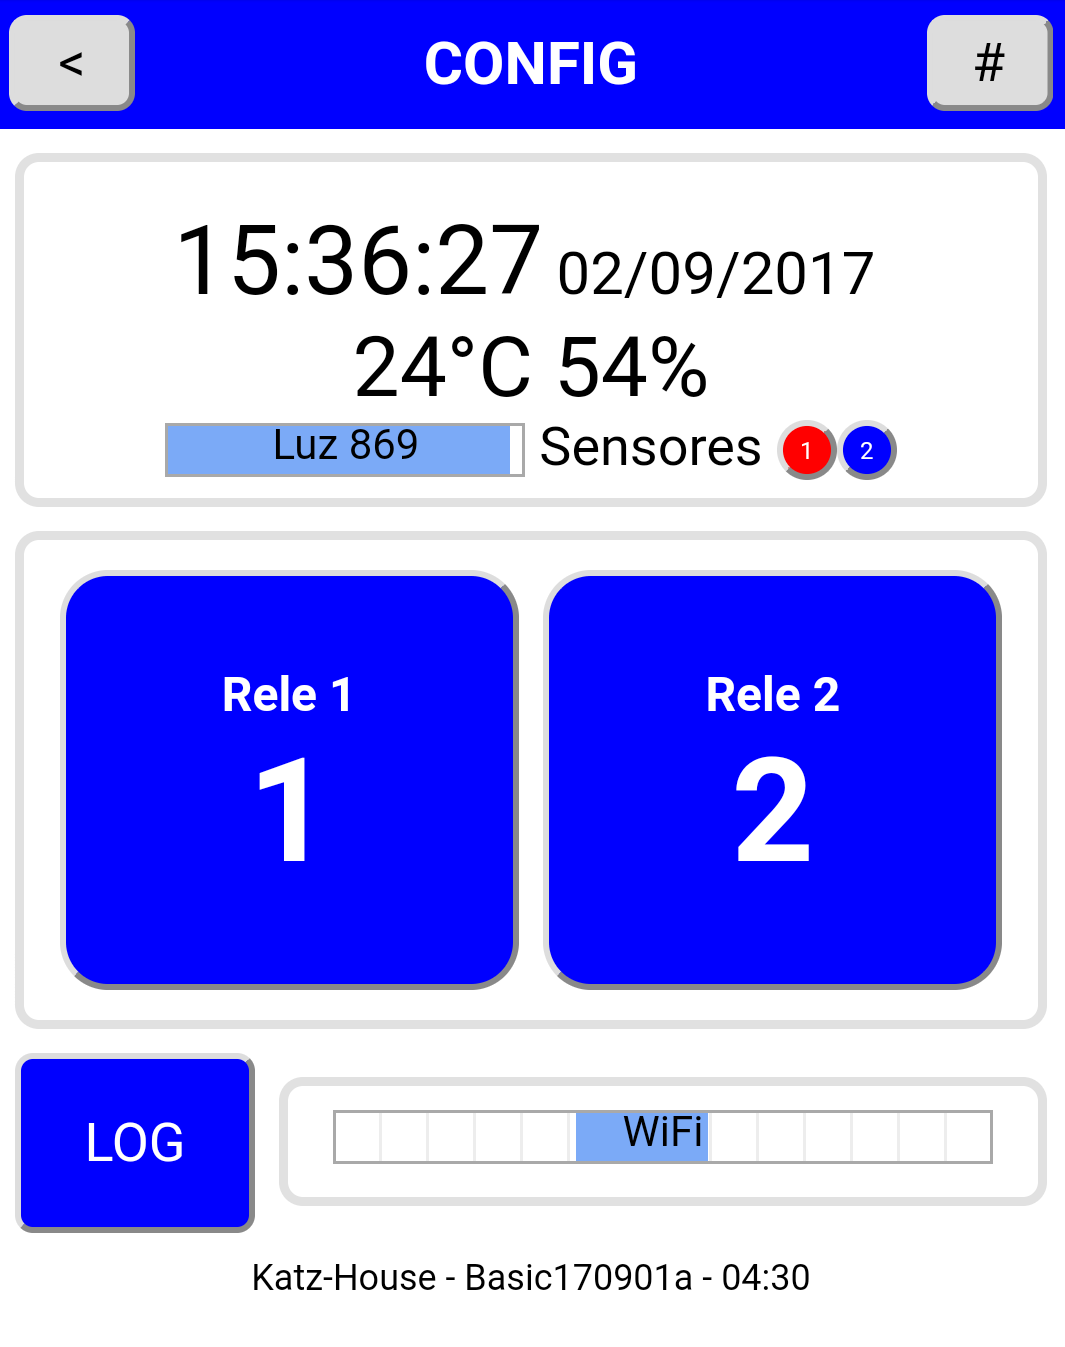
\includegraphics[height=6cm]{menuPrincipalBackup}
        \label{fig:menuPrincipalBackup}
    \end{minipage}
    \hfill
    \begin{minipage}{.4\linewidth}
        \centering
        \captionof{figure}{Teclado para digitação da senha}
        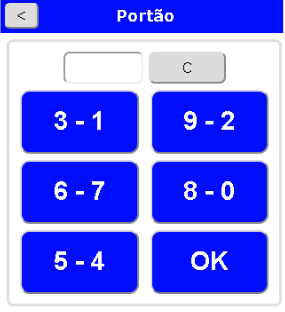
\includegraphics[height=6cm]{senhaBackup}
        \label{fig:senhaBackup}
    \end{minipage}
\end{figure}

No caso de proteção de controle por senha, é exibido o painel numérico como na Figura \ref{fig:senhaBackup}. A cada requisição da página, o módulo manda um mapeamento das teclas diferente. Por exemplo, de teclas A, B, C, etc. para (3,1), (9,2), etc. Após o usuário entrar com a senha (sequência de teclas do tipo A, B, C, etc.), o módulo valida a sequência e autoriza o acionamento. Dessa forma, pessoas não conseguem copiar a senha ao visualizar a sequência de teclas do usuário, tampouco um invasor poderia copiar a sequência e utilizá-la para abertura logo em seguida, pois o mapeamento seria outro.

\subsection{Configurações}

A partir do menu principal do módulo, pode-se ter acesso ao seu log para depuração, uma opção disponível apenas para administradores, e um menu de configurações. Do menu de configurações, pode-se alterar o modo do display (dentre 3 opções) e as cores do módulo, conforme opções anteriormente citadas.

Ainda do menu de configurações, podem-se configurar alertas e alarmes (sonoros a partir dos módulos e pela Internet através do provedor gratuito Blynk e email), relés (possibilidade de auto ligar a partir de um sensor específico ou de ser acionado a partir de um sinal de rádio - usualmente um controle remoto ou até um sensor de abertura adicional ou mais de uma opação) e o log (quais parâmetros são persistidos e mandados para a nuvem). Também pode-se acessar o menu de Ferramentas, no qual é possível realizar testes de \emph{auto reset} para verificação do funcionamento do circuito antitravamento, que age em cerca de 30 segundos, reiniciar o módulo, desconectá-lo, voltar à versão de fábrica (versão implementada em software, enquanto a versão em hardware é realizada por meio de botão oculto) e atualizar o \emph{firmware} (apenas disponível para administradores).
Ao acessar a atualização de \emph{firmware}, escolhe-se a opção, que mostra a versão atual e, após escolha do arquivo, a versão a ser inserida. % TODO melhorar essa frase

É possível também acessar as configurações avançadas \ref{fig:firmwareconfigavancadasDHT}. Nela, pode-se configurar um offset para temperatura e umidade, de preferência realizados a partir de um medidor confiável para calibração.

Do menu de configurações avançadas, podem ser configurados os sensores e controladores de radiofrequência (sem fio), aspectos de conectividade do servidor gratuito Blynk e possivelmente trocar a rede Wi-Fi em que o módulo está conectado. Ainda, para administradores, há a opção de configurar os usuários que têm acesso ao módulo.

Ainda pode-se trocar o nome do módulo e ativar/desativar o ponto de acesso (para acesso direto ao módulo), além de configurar o nome (SSID) e senha de sua rede Wi-Fi.

Demais ilustrações referentes às configurações do aplicativo backup estão disponíveis no Anexo \ref{attachmentsImagensBackup}{}.

\subsection{Abertura de porta do roteador}

Para acessar o módulo e o menu remotamente, um solução é usar a abertura de porta (mecanismo NAT ou \emph{virtual servers}), configurável nas páginas de configuração dos roteadores. Maiores informações para essa configuração podem ser encontradas nos manuais dos roteadores. Observe que há uma segurança menor envolvida com essa configuração. Assim, essa alternativa provê a abertura da porta para acesso remoto sem a necessidade de serviços em nuvem, o que é indicado apenas para usuários que podem lidar com um nível de segurança mais baixo.

\begin{figure}[hbp]
    \centering
    \caption{Página de configuração TP Link}
    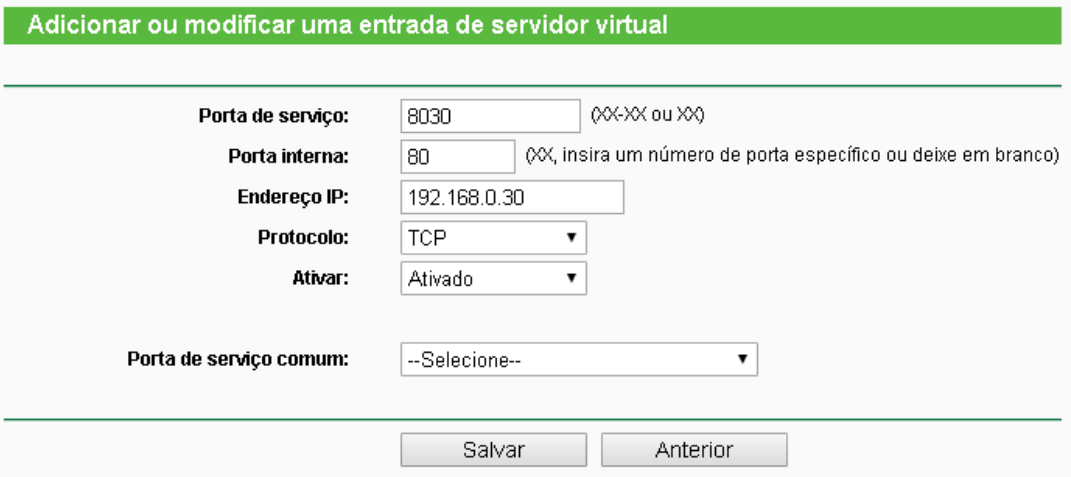
\includegraphics[width=0.8\textwidth]{tpLinkAppBackup}
    \label{fig:tpLinkAppBackup}
\end{figure}

\emph{Obs.:} Caso sua operadora só forneça o CGNAT, a abertura de porta por parte do usuário não será possível.

\subsection{Controle remoto}

Para que o controle remoto seja corretamente configurado, são necessários os seguintes passos:
\begin{enumerate}
    \item
    A partir da página inicial do módulo, entre em \# \textrightarrow{} Configurações Avançadas \textrightarrow{} RF433.

    \item
    Configure o Sensor de Abertura “Sulton” no modo 2 para mandar sinais diferentes de abertura e fechamento. Consulte o manual do fabricante.

    \item
    Aperte +, espere até a página indicar “Aguardando” e abra o sensor de abertura. É permitido incluir diversos sinais para o controle do mesmo relé, abertura ou fechamento de sensor. Aperte “OK” no canto superior direito da página, para salvar suas configurações.

    \item
    Repita o passo 3 para o fechamento do sensor de abertura. \textbf{Cuidado:} o sensor de abertura repete algumas vezes o mesmo sinal. Aguarde alguns instantes entre gravar a abertura e o fechamento para não gravar o mesmo sinal. Isso pode ser verificado na série numérica que aparece gravada: se estiver igual, há um problema.

    \item
        \begin{enumerate}
            \item
            A partir da página inicial do módulo, entre em \# \textrightarrow{} Configurações Avançadas \textrightarrow{} RF433.

            \item
            Aperte + (ao lado do relé 1 ou relé 2), espere até a página indicar “Aguardando” e abra o sensor de abertura. É permitido incluir diversos sinais para o controle do mesmo relé, abertura ou fechamento de sensor).

            \item
            Aperte "OK" no canto superior direito da página para salvar suas configurações.

        \end{enumerate}
\end{enumerate}

\subsection{Notificações}
Para que as notificações sejam ativadas, siga os próximos passos.

\begin{enumerate}
    \item
    Para que o suporte consiga acessar remotamente o módulo e realize a coleta de dados, acesse \# \textrightarrow{} Configurações Avançadas.\textrightarrow{} Blynk.

    \item
    Insira o \emph{Auth Token} (e.g. aa7a6dc1170640f08e951ed8cd2198a1).

    \item
    Selecione Notificações ao iniciar: Sim, e Wi-Fi: Sim.

    \item
    Aperte em OK, no canto superior direito, para salvar suas alterações.
\end{enumerate}

\subsection{Offset de temperatura e umidade}

\begin{enumerate}
    \item
    Para que o suporte consiga acessar remotamente o módulo e realize a coleta de dados, acesse \# \textrightarrow{} Configurações Avançadas.\textrightarrow{} Temperatura e Umidade.

    \item
    Efetue a calibração do equipamento usando uma referência externa.

    \item
    Aperte em OK, no canto superior direito, para salvar suas alterações.
\end{enumerate}

\subsection{\emph{Hard reset}}
\begin{enumerate}
	\item Ligue na tomada
	\item Abra a tampa do módulo, e retire o isopor que cobre o sensor de temperatura azul;
	\item Localize o botão (“\emph{pushbutton}”), após retirar o isopor;
	\item Pressione o botão até ouvir 6 bipes;
	\item O módulo retornará para a configuração de fábrica. Veja as seções a seguir para sua configuração inicial.
\end{enumerate}

\subsection{Setup inicial}
\begin{enumerate}
	\item Primeiro, conecte à rede Wi-Fi do Módulo, com nome CONFIG (a senha da rede CONFIG é 12345678).
	\item Abra um navegador e vá ao endereço 192.168.4.1 para entrar na página de configuração. Entre com as credenciais (login: admin e senha: 1234).
	\item Espere até que as redes disponíveis apareçam, selecione a rede de sua casa e forneça sua senha para conectar o módulo à Internet.
	\item Observe o endereço local 192.168.0.X que aparecerá no LCD do módulo. Caso não consiga ver, realize o passo 7 e use uma ferramenta como o “Zentri” (aplicativo Android) para descobrir em que endereço o módulo entrou. Para ver na tela novamente, pode-se tirar o módulo da tomada e ligá-lo novamente.
	\item Espere o módulo reiniciar (continue na rede CONFIG) e aguarde até a página recarregar. Insira o nome do módulo e depois aperte “Salvar e Reiniciar”.
	\item Conecte-se novamente na rede Wi-Fi da sua casa.
	\item Entre no endereço 192.168.0.X que foi mostrado no módulo, clique em \# e então em “Reiniciar Busca”. Aguarde até que todos os módulos sejam descobertos.
	\item Retorne para a página anterior (usando o “\textless” no canto superior esquerdo). Você verá o menu principal da casa, e então poderá controlar relés, visualizar dados coletados pelos módulos e entrar em cada módulo. O menu é personalizado na página anterior (ao pressionar o “\#” no canto superior direito da tela).
\end{enumerate}
